\section{World models}
\label{sec:architectures}
\label{sec:training}

%%SL.12.27: Perhaps organizationally it would be better to first have a top-level Overview section to describe the parts of the method, and then a single top-level section with the name of the method, with subsections about the individual parts of the method? If the goal of this section is to discuss predictive model architectures, perhaps that would also make for a better section title: Predictive Model Architectures or something? The title of the first paragraph "Architecture of a Neural Simulator" could also work well (note however that in the deep learning community, "neural simulator" sometimes takes on a very specific meaning as an object-decomposed model that emulates the high-level design of a physics simulator)

% Dumitru. here is how I would structure this: 1-2 sentences about what we are looking for in a world model (stochasticity, scalability, stability). Say that to this end we came up with a new architecture that is straightforward but that is novel for video prediction. Also say that we compare with SV2P, and describe it. Then go into the details of the filter sizes and training losses: first the stuff that is common to both, then the specifics for each model. Alternative proposal is to describe the details of the world model training that are common first, and then describe the models themselves.}

%%SL.12.27: It could be a good idea at the beginning of this paragraph to explain the problems that the architecture design is trying to address so as to motivate the design decisions.
\paragraph{Architecture of a neural simulator of an environment. } Our basic architecture, presented in Figure~\ref{fig:kanapa}, resembles the convolutional feedforward network from \cite{video_prediction}.  The input $X$ consists of a few consecutive game frames and an action $a$. The visual input is processed by stacked convolution layers. The actions are one-hot-encoded and embedded in a vector which is multiplied channel-wise with the output of the conv layers. It is then processed by fully connected layers and deconvolved. The network outputs the next frame of the game and the value of reward.% Predicted rewards in \pong are $-1,0,1$ and are the same as in the original ALE environment (see Section \ref{sec:envs}). Predicted rewards  \breakout\ are $0$ and $1$: every positive reward is considered as $1$. Predicted rewards in the dense version of \freeway\ are $0$, $0.01$ and $1$. % We truncate rewards to $3$ possible values $in \pong:

	In most of our experiments we choose the input to be four frames as with our choice of environments they fully identify the state of the game. The network is the workhorse of our simulated environment $env'$. The environment contains a memory $M$ of four frames, which is initialized with frames retrieved for the original environment. Given an action $a$ the tuple $(M,a)$ is processed by the network outputting a new frame and a reward $r$. The oldest frame of $M$ is discarded and the new one is included. 

%\todo{pm: The next section is too much of storytelling}
%\todo{you can shorten it and put the rest of details as a table}
% As shown in model-free experiments \cite{dqn,dqn2,ppo,acktr,rainbow,a3c}, using $4$ frames seems to be sufficient to train agents in a majority of Atari games and the same design decision we applied to neural network simulators. % the case of training of
% % Why $4$ frames? It is enough for reinforcement learning in many games.
% % Since in this work
% Another design decision concerned resizing and possible augmentation of the input frame marked as $X$ in Figure \ref{fig:kanapa}. We decided to feed the original $4$ RGB frames of the size $160\times 210$ pixels, meaning that a single input to the neural network is a tensor of the size $4 \times 160\times 210\times 3$ with a single cell of the tensor ranging from $0$ to $255$. In our design the same is true about the ouput $X'$.
%\todo{Important: no pooling}

In our experiments we varied details of the architecture above. In most cases we use a stack of four conv layers with $64$ filters followed by three dense layers (the first two have $1024$ neurons). The dense layers are concatenated with $64$ dimensional vector with a learnable action embedding. Next, three deconv layers of $64$ filters follow. An additional, final, deconv layer outputs an image of the original $210\times 160$ size. The number of filters is either $3$ or $2\times 256$. In the first case the output is a real-valued approximation of pixel's RGB value. In the second case filters are followed by softmax producing probability distribution on the color space. The reward is predicted by a softmax attached to the last fully connected layer. 
We used dropout equal to $0.2$ and the layer normalization. 

We have also experimented with Stochastic Variation Video Prediction (SV2P)~\cite{sv2p}, a recent technique that incorporates a latent variable model with a generative recurrent network. The latter is a convolutional LSTM from \cite{cdna} that internally predicts transformations of the context images conditioned on latent values, actions and the previous frames. The model is trained with the reparametrization trick and allows for efficient inference at test time. When successfully trained, it make it possible to sample diverse and plausible action-conditioned futures. For the Atari experiments, we followed the same protocol of training as with the basic convolutional model described above. Note that generally speaking the multiplier for the KL-loss $\beta$ has to be tuned on a per-game basis: we tried 3 such values per game (TODO: confirm with mbz how many we actually tried).\todo[inline]{The reference to KL-loss may require some elaboration or abstraction.}

% MB.1.17 commenting this out
% \begin{figure}[H]
% \centering
% 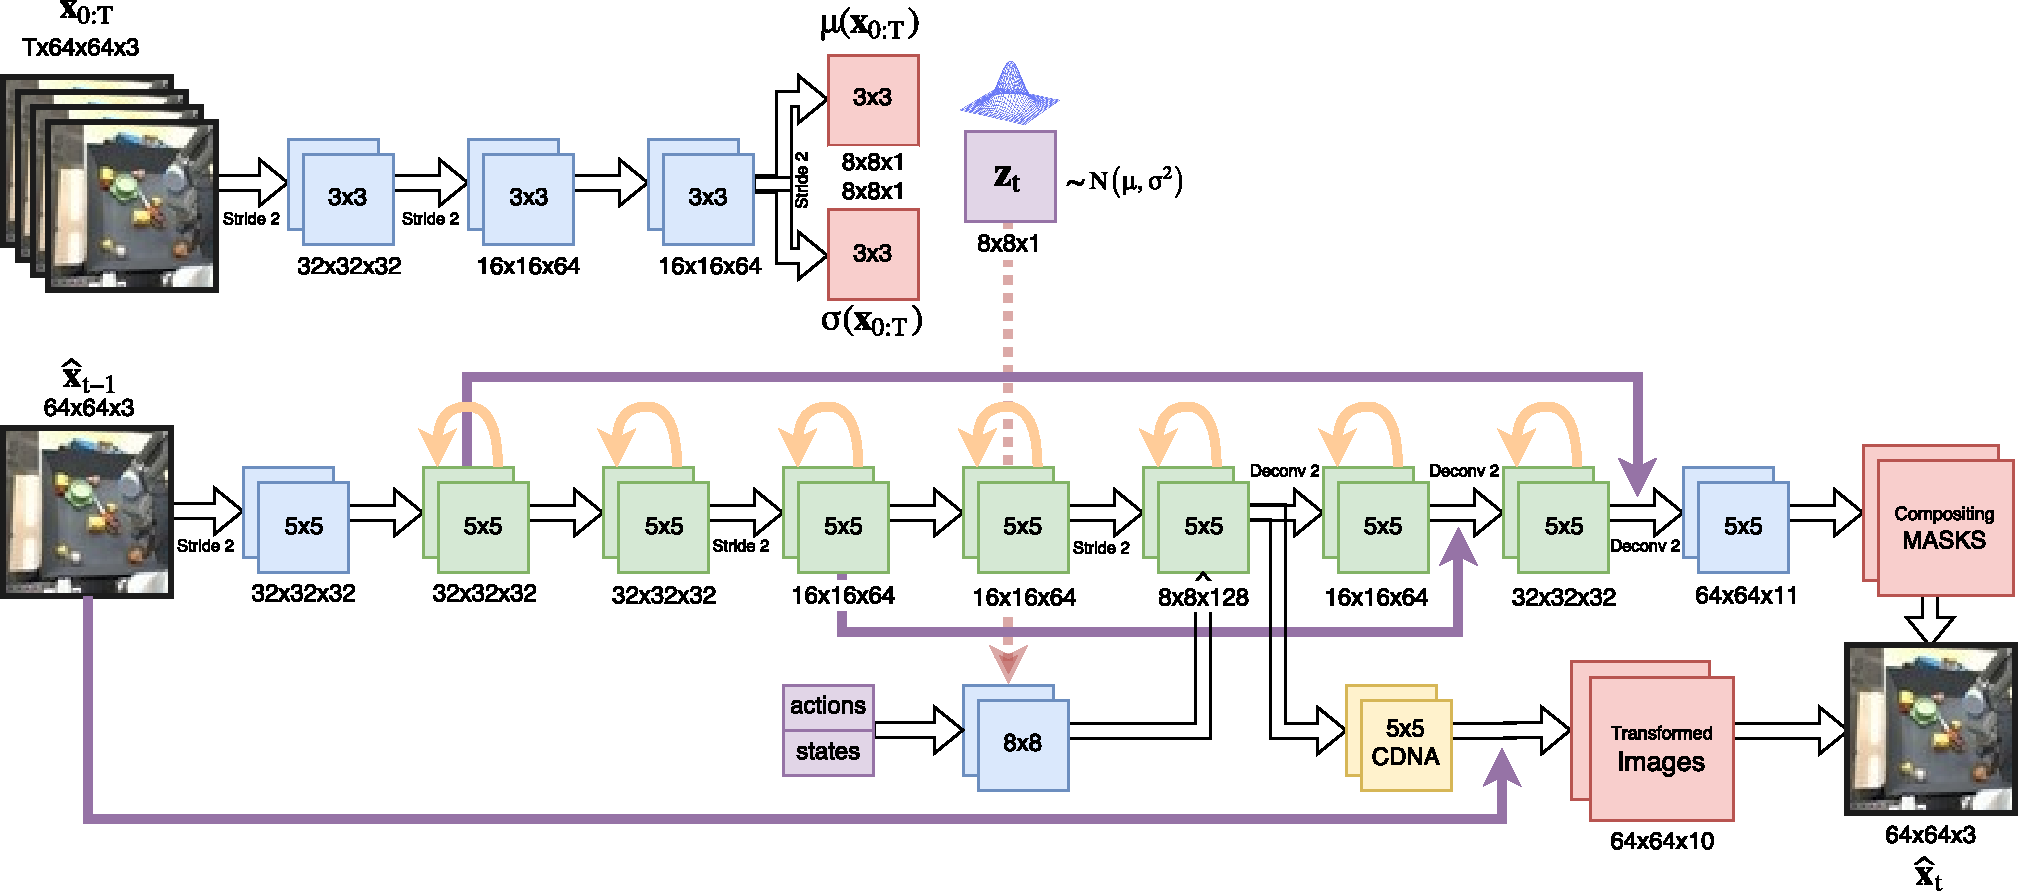
\includegraphics[width=3.5in]{figures/sv2p}
% \caption{The Stochastic Variational Video Prediction model (SV2P) by \cite{sv2p}}
% \label{fig:sv2p}
% \end{figure} 

\paragraph{Loss functions}
The visual output of our networks are either one float per pixel/channel or the categorical 256-dimensional softmax. 
In the case of the real output we used the \textit{clipped $L_2$ loss}, viz. $\max(x^2 - C, 0), C>0$. We found that clipping was crucial for improving prediction power of the models (both measured with the correct rewards predictions per sequence metric and successful trainings using Algorithm \ref{dpll}). We conjecture that the clipping substantially decreases the magnitude of gradients stemming from fine-tuning of big areas of background consequently letting the optimization process to concentrate on small but important areas (e.g. the ball in Pong). Setting $C$ corresponding to $10$ pixels worked particularly well in our experiments. 
We used similar trick for the softmax outputs, namely we clipped the cross-entropy loss once the model achieved high level of confidence about a pixel value (we used $98\%$ in our experiments). As in the first case, clipping was crucial for obtaining well performing models. 

\paragraph{Scheduled sampling}
By design, the clipped loss does not produce accurate pictures. The simulator $env'$ consumes its own predictions from previous steps thus, due to compounding errors, the model may drift out of the area of its applicability. We mitigate this problem by randomly replacing in training some frames of the input $X$ by one step predictions. Typically, we increase the mixing probability during training arriving to $50\%$. 

\begin{figure*}[t]
\centering
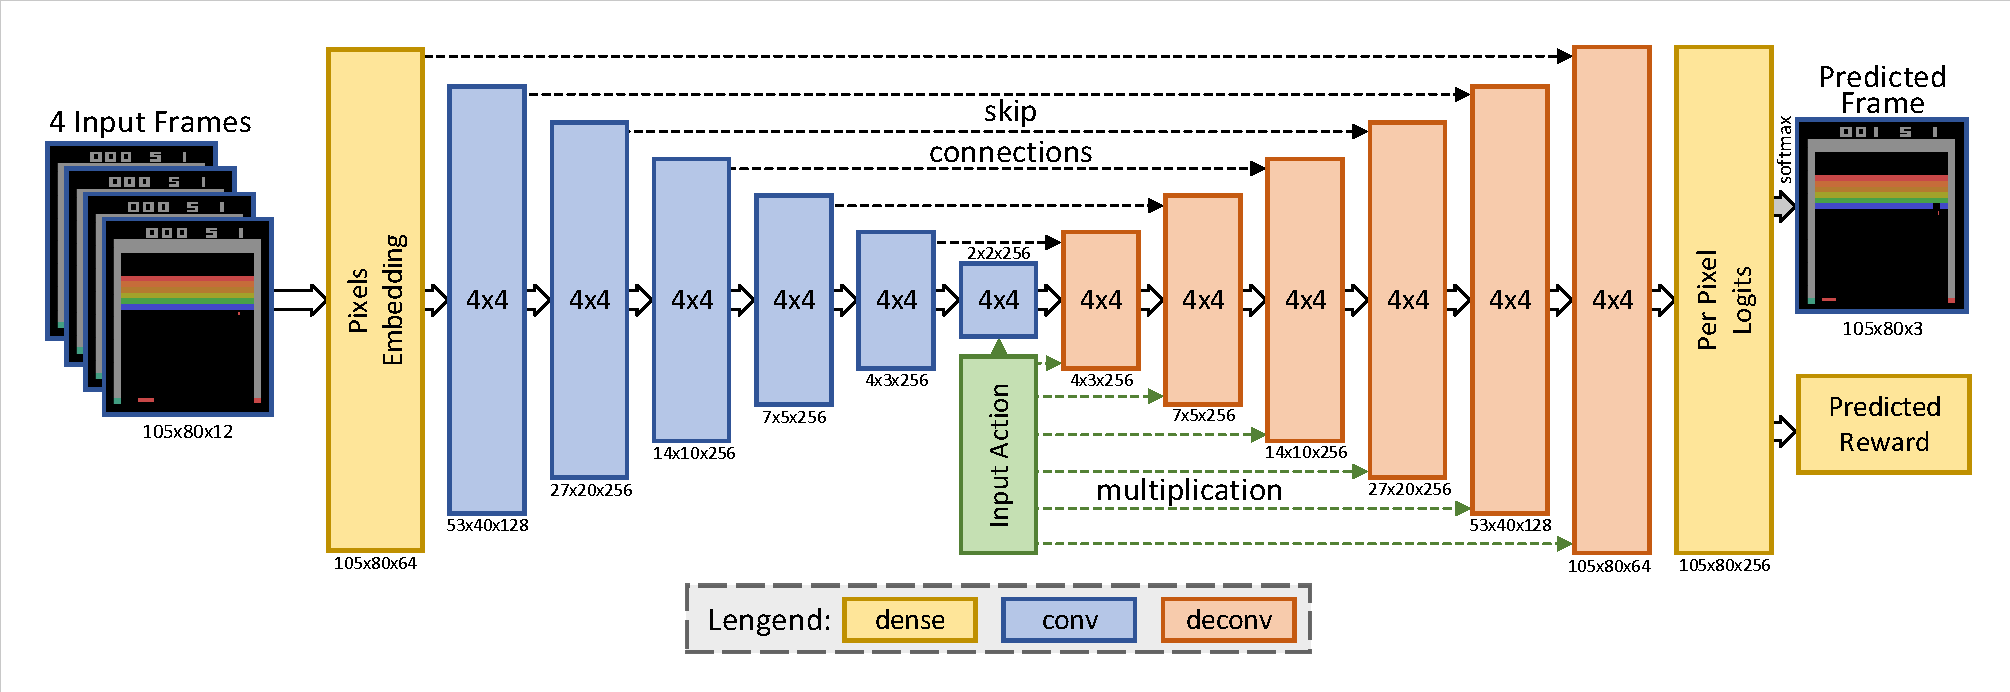
\includegraphics[width=0.8\textwidth]{figures/model_basic_det.pdf}
\caption{Architecture of deterministic model which consists of a skip-connected convolutional encoder and decoder. The input to the model is four stacked frames as well as the selected action while the output is the next predicted frame and expected reward. Input pixels and action are embedded using fully connected layers and there is per-pixel softmax ($256$ colors) in the output.}
\label{fig:model_det}
\end{figure*}

\begin{figure*}[t]
\centering
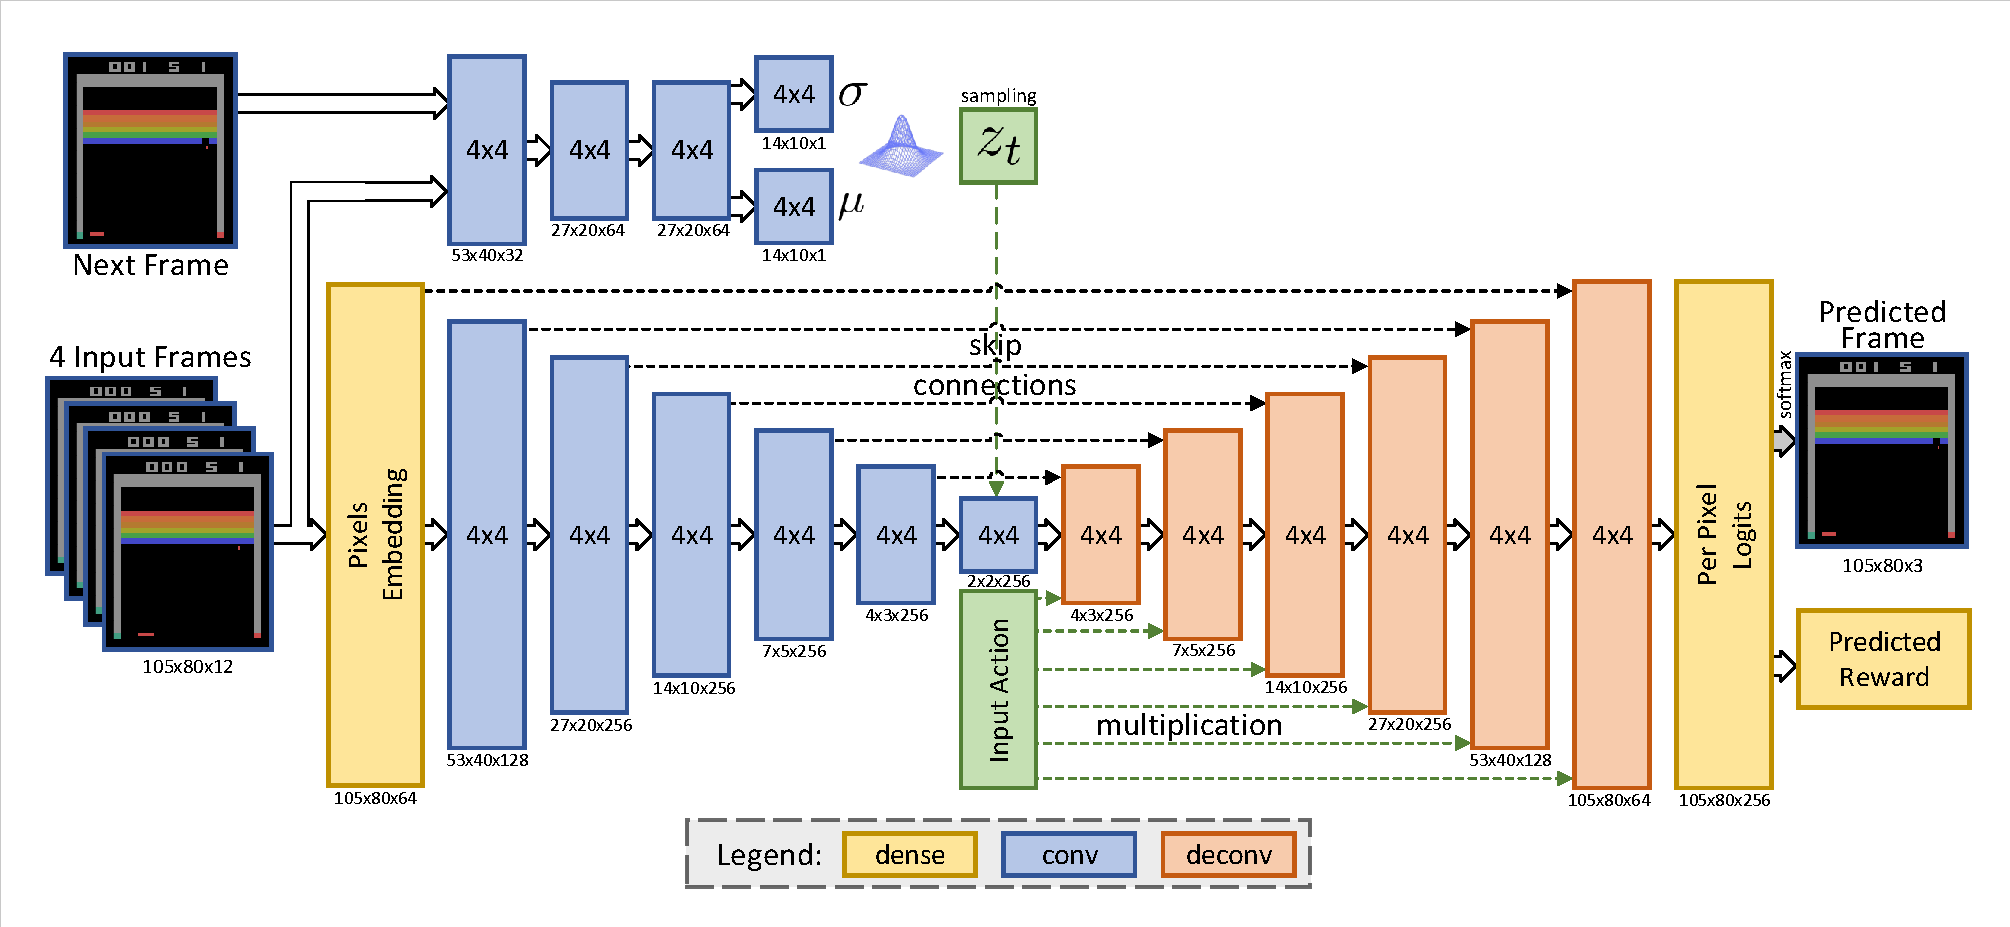
\includegraphics[width=0.8\textwidth]{figures/model_basic_stoch.pdf}
\caption{Architecture of stochastic model. The generative network is the same as Figure~\ref{fig:model_det} with an additional convolutional inference network to approximates the posterior given the next frame. The latent values will be sampled from approximated posterior and an assumed prior of $\mathcal{N}(\mathbf{0}, \mathbf{I})$ at training and inference time respectively.}
\label{fig:model_stoch}
\end{figure*}

\begin{figure*}[t]
\centering
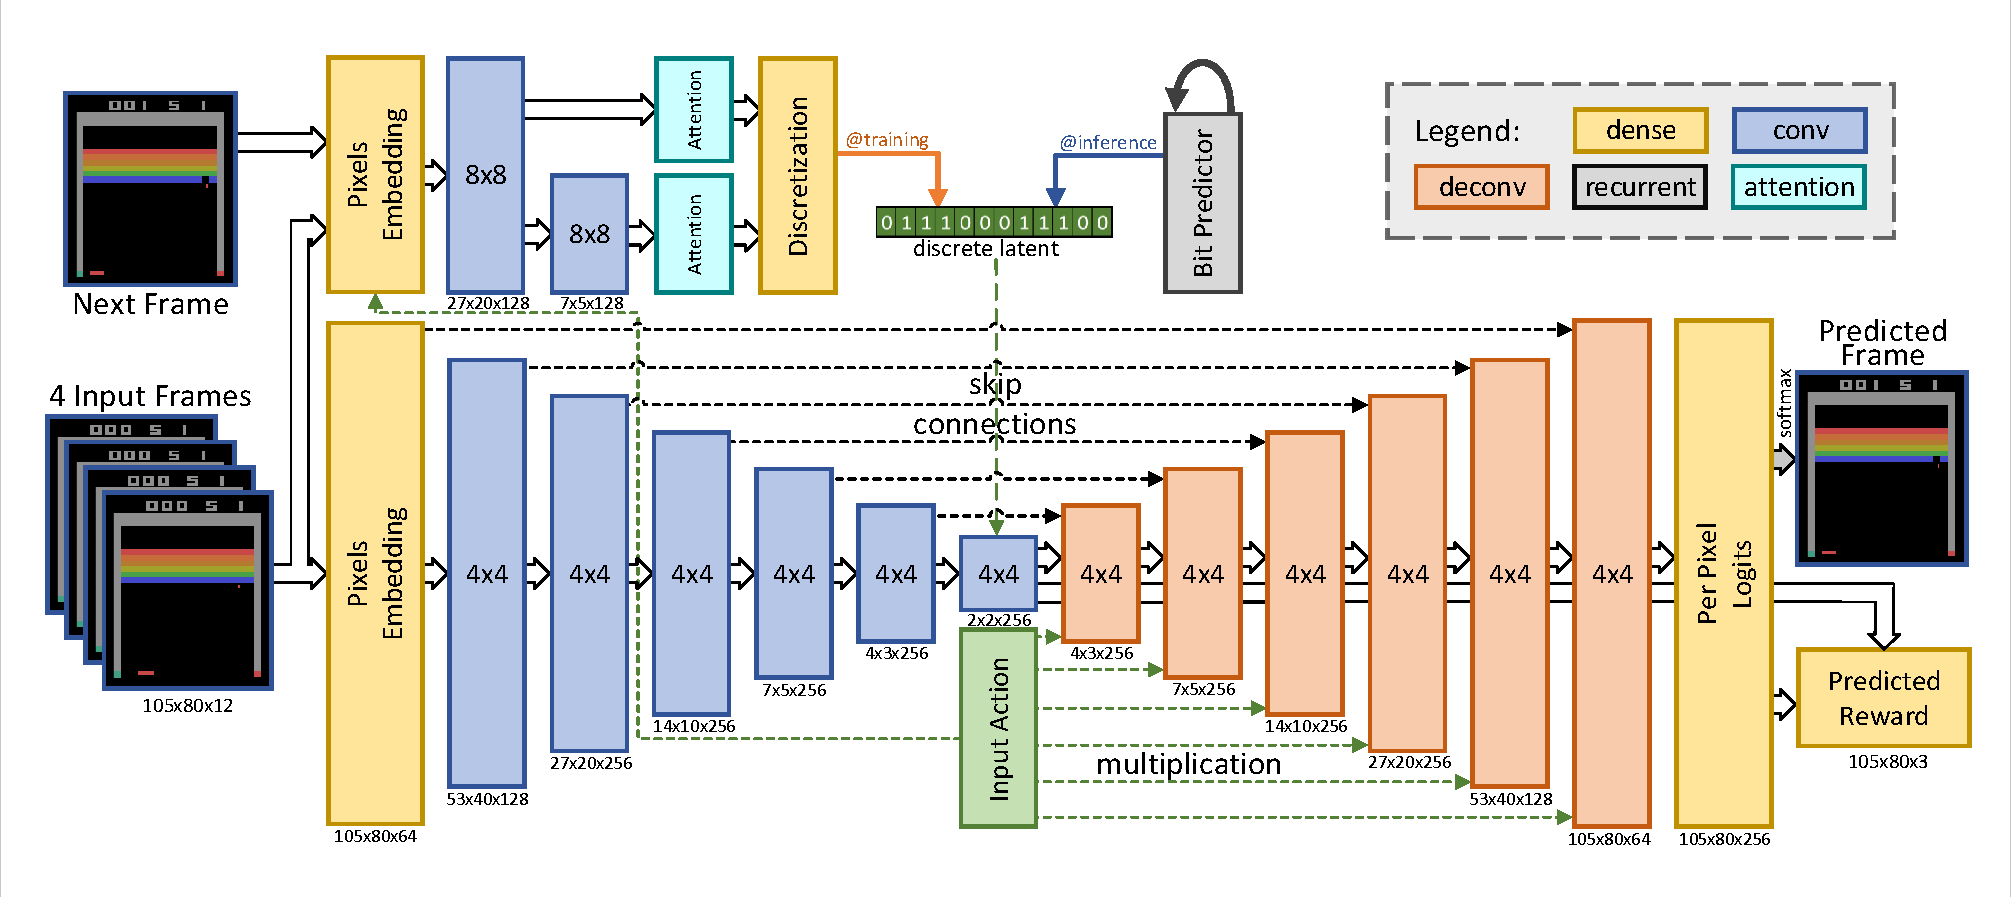
\includegraphics[width=0.8\textwidth]{figures/model_basic_disc.pdf}
\caption{Architecture of stochastic model with discrete latent. The overall architecture of this models is similar to Figure~\ref{fig:model_stoch} with two main differences. First, at training time, the sampled latent values from the approximated posterior will be discretized into bits. The backpropagation bypasses the discretization similar to~\citet{van2017neural}. A third LSTM based network is trained to approximate each bit given the previous ones. At inference network, the latent bits are predicted auto-regressively using this network.} 
\label{fig:full_discrete}
\end{figure*}



% \section{Design and training of simulators}
% \label{sec:architectures}

% \paragraph{Architecture of a neural simulator of an environment. } Our basic architecture, see Figure \ref{fig:kanapa}, resembles the convolutional {\em feedforward} architecture from \cite{video_prediction}.  The input $X$ consists of $4$ game frames and the action $a$. The visual input is processed by stacked convolution layers. The actions are one-hot-encoded and then embedded in a vector which is concatenated with the the output of the conv layers. It is then processed by some fully connected layers and deconvolved. The output of the network is the next gameframe and the value of reward. Predicted rewards in \pong are $-1,0,1$ and are the same as in the original ALE environment (see Section \ref{sec:envs}). Predicted rewards  \breakout\ are $0$ and $1$: every positive reward is considered as $1$. Predicted rewards in the dense version of \freeway\ are $0$, $0.01$ and $1$. % We truncate rewards to $3$ possible values $in \pong:

% %\todo{pm: The next section is too much of storytelling}
% %\todo{you can shorten it and put the rest of details as a table}
% As shown in model-free experiments \cite{dqn,dqn2,ppo,acktr,rainbow,a3c}, using $4$ frames seems to be sufficient to train agents in a majority of Atari games and the same design decision we applied to neural network simulators. % the case of training of
% % Why $4$ frames? It is enough for reinforcement learning in many games. 
% % Since in this work
% Another design decision concerned resizing and possible augmentation of the input frame marked as $X$ in Figure \ref{fig:kanapa}. We decided to feed the original $4$ RGB frames of the size $160\times 210$ pixels, meaning that a single input to the neural network is a tensor of the size $4 \times 160\times 210\times 3$ with a single cell of the tensor ranging from $0$ to $255$. In our design the same is true about the ouput $X'$. 
% %\todo{Important: no pooling}

% In our experiments we varied a number of layers, but the most standard architecture of the encoder consists of $4$ convolutional layers with 128 filters, followed by 3 dense layers. The third of the layers marked as $e$ in Figure \ref{fig:kanapa} is stacked with the embedding of actions marked as $a$ in Figure \ref{fig:kanapa}. The stacked layer is followed by $4$ deconvolutions.     

% \paragraph{Metrics}
% In our work we mostly abandonded $L_2$ metric as a measure of accurracy. We argue that in many cases it is not well suited to asses the models as it underweights meaning small (but potentially crucial) objects. Instead we introduce \textit{correct rewards per sequence} parametrized by the sequence length $n$. By definition the metric is the ratio of action sequences in the training/eval set for with $env'$ predicts total reward consistent with the one of $env$.

% \paragraph{Loss functions}
% Our experiments followed two lines. The first output was a single real value for each pixel and channel, in the second we used categorical output of 256-dimensional softmax. 

% For both losses we introduced a clipping factor: the final loss was $\max(loss - C, 0)$ for a constant $C>0$. We found that clipping was crucial for improving prediction power both over the standard $L_2$ loss and over the standard cross-entropy loss. We conjecture fine-tuneing of big areas of background the clipping substantially decreases the magnitued of gradients stemming from fine-tuneing of big areas of background consequnetly letting the optimisation process to concentrate on small but important areas, like the ball in Pong. We used $C = 0.01$ for cross-entropy loss (so the model did not get any benefit from being more than 99\% confident about any pixel value) and $C = 10$ for $L_2$ loss so
% that being within $3$ RGB values was considered sufficient.

% \paragraph{Mixing.} \todo{Add mixing}

% \paragraph{Resets.} \todo{Add resets}



%\cite{video_prediction,recurrent}. 
%Important points: the encoder-decoder architecture, prediction-dependent transition, observation-dependent transition, long-short term accuracy. 

%\paragraph{Training of a simulator of an environment}
%Some decisions.
%\todo[inline]{which models we want to discuss? Loss functions, layer details, mixing, metrics such as percent of successful trajectory-reward predictions, {\bf negative mining} (Henryk) Yes, we want to discuss, details of training to be described by Piotr}

%\begin{figure}
\begin{tikzpicture}[scale=0.1,every node/.style={scale=0.1}]]

	\node (1) [draw, dashed, minimum height=15em, minimum width=62em, xshift=24em, fill=olivegreen, fill opacity=0.2, very thick, rectangle, rounded corners] {};
		\node (la1) [below=0em of 1] {{\emph{encoder}}};
	\node (2) [draw, dashed, minimum height=14em, fill = red, fill opacity=0.2,minimum width=35em, xshift=63.5em, very thick, rectangle, rounded corners] {};
		\node (la1) [below=0em of 2] {{\emph{decoder}}};

	\node[] (i2) {};
	\pic[fill=green!50] (I2) {cube={1.8/1.8/0.4/1}};
	
	\togglefalse{redraw}
	\togglefalse{redraw2}
	
  	\node[right=16em of i2] (y) {};
  	
  	\pic[right=16em of i2, fill=echoreg!50] (Y) {cube={1.8/1.8/1/1}};
  	
  	\node[right=12em of y] (y1) {};
  	\pic[right=12em of y, fill=red!50] (Y1) {cube={0.9/0.9/1/1}};
  	
  	\node[right=12em of y1] (y2) {};
  	\pic[right=12em of y1, fill=echoreg!50] (Y2) {cube={0.9/0.9/2/1}};
  	\node[right=10em of y2] (y3) {};
  	\pic[right=10em of y2, fill=red!50] (Y3) {cube={0.45/0.45/2/1}};
  	
  	\node[right=9em of y3] (z1) {};
  	\pic[right=9em of y3, fill=mymauve!50] (Z1) {cube={0.9/0.9/1/1}};
  	
  	\node[right=12em of z1] (z2) {};
  	\pic[right=12em of z1, fill=mymauve!50] (Z2) {cube={1.8/1.8/0.4/1}};
  	
  	\draw [-stealth, ultra thick] (I2-B) -- node[above] {Conv.} node[below] {ReLU} (Y-A);
  	
  	\draw [-stealth, ultra thick] (Y-B) -- node[above] {Pool} (Y1-A);
  	
  	\draw [-stealth, ultra thick] (Y1-B) -- node[above=0.3em, inner sep=0.1em] {Conv.} node[below] {ReLU} (Y2-A);
  
  	\draw [-stealth, ultra thick] (Y2-B) -- node[above] {Pool} (Y3-A);
  	
  	
  	\draw [-stealth, ultra thick] (Y3-B) -- node[above] {Deconv.} node[below] {ReLU} (Z1-A);
  	
  	\draw [-stealth, ultra thick] (Z1-B) -- node[above] {Deconv.} node[below] {logistic} (Z2-A);
  	
  	
  	\color{black}
  	
  	\toggletrue{redraw}
  	\toggletrue{redraw2}
  	
  	\node[right=16em of i2] (y) {};
  	\pic[right=16em of i2, fill=echoreg!50] (Y) {cube={1.8/1.8/1/1}};
  	
  	\pic[right=12em of y, fill=red!50] (Y1) {cube={0.9/0.9/1/1}};
  	
  	\pic[right=12em of y1, fill=echoreg!50] (Y2) {cube={0.9/0.9/2/1}};
  	
  	\pic[right=9em of y3, fill=mymauve!50] (Z1) {cube={0.9/0.9/1/1}};
  	
  	\togglefalse{redraw2}
  	
  	\pic[right=10em of y2, fill=red!50] (Y3) {cube={0.45/0.45/2/1}};
  	
  	\toggletrue{redraw2}
  	
	\node[] (i2) {\LARGE ${\bf X}$};
  	\node[right=9.25em of y2] (y3) {\LARGE ${\bf z}$};
  	\node[right=11em of z1] (z2) {\LARGE ${\bf X}'$};

\end{tikzpicture}
\label{fig:kanapa_net}
\end{figure}
% source: https://raw.githubusercontent.com/PetarV-/TikZ/master/Convolutional%20autoencoder/convolutional_autoencoder.tex
% overleaf copy (can be modified): https://www.overleaf.com/16266360vmyxnwdwdnpn

%Do we want a figure like\todo{The figure is missing actions and rewards, but this can be fixed}
% \begin{figure}[H]
% \centering
% 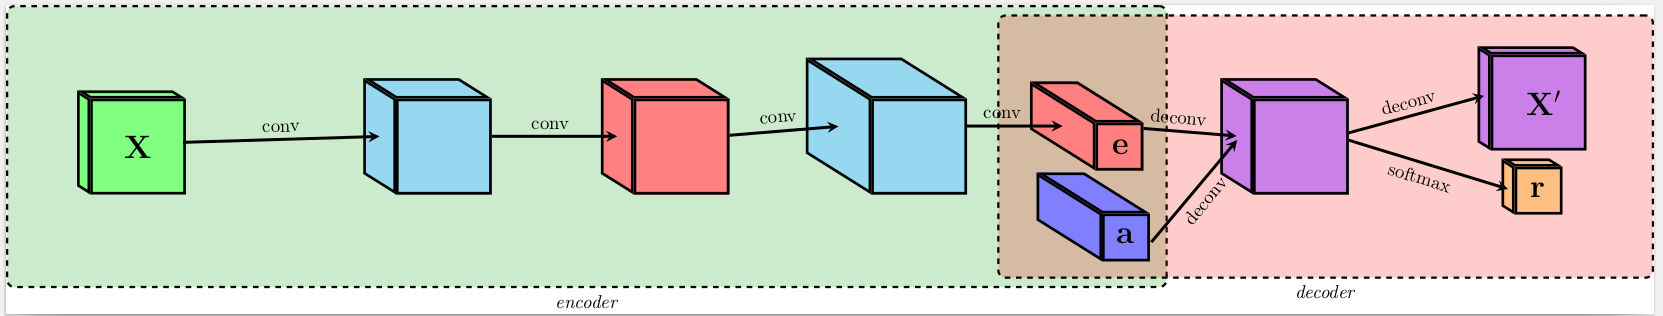
\includegraphics[width=5.5in]{figures/new_arch.png}
% \caption{A simplified view of our encoder-decoder architecture.}
% \label{fig:kanapa}
% \end{figure}

